\documentclass[french, 11pt]{article}

\input{setup.tex}

\def\chapitre{5}
\def\pagetitle{Fils d'exécution.}

\begin{document}

\input{title.tex}

\begin{defi}{Processus.}{}
    Un \bf{processus} un programme en cours d'exécution sur un ordinateur.\\
    Il possède une mémoire allouée et des ressources.
\end{defi}

\begin{defi}{Fil d'exécution.}{}
    Un \bf{fil d'exécution} est un processus pouvant être exécuté en parallèle d'autres fils.
\end{defi}

\begin{defi}{Section critique.}{}
    Une \bf{section critique} est une portion d'un programme qui ne doit être exécutée que par un nombre limité de fils à la fois.
\end{defi}

\begin{defi}{Algorithme de Peterson.}{}
    Dans une situation avec deux fils, on cherche à garantir l'exclusion mutuelle.\\
    Pour que chaque fil possède son propre identifiant, on le lui fournit lors de l'appel de la fonction qu'il doit exécuter.\\
    On suppose qu'on a un fil d'identifiant 0 et un fil d'identifiant 1 et qu'ils partagent un tableau \texttt{veut\_rentrer} de taille 2 et une variable \texttt{tour}.\\
    Avant la section critique :
    \begin{pygmented}[lang=c, hidealllines=true, linenos=true]
        veut_rentrer[id] = true;
        tour = 1 - id;
        while (tour != id && veut_rentrer[1-id]) {}
        section critique
    \end{pygmented}
    Après la section critique : \c{veut_rentrer[id] = false;}\\
    Un fil peut rentrer en section critique si c'est son tour ou si l'autre fil ne souhaite pas rentrer.
\end{defi}

\vspace*{-0.7cm}

\begin{prop}{}{}
    Cet algorithme garantit l'exclusion mutuelle.
    \tcblower
    Raisonnons par l'absurde et supposons que les deux fils soient en section critique.\\
    Les deux cases de \texttt{veut\_rentrer} sont à \c{true}. On considère $f_i$ le dernier fil à être rentré en section critique.\\
    Alors $f_i$ a pu rentrer car \texttt{tour} valait $i$, donc $f_j$ a modifié \texttt{tour} en dernier.\\
    Avant de modifier \texttt{tour}, $f_i$ a modifié \texttt{veut\_entrer[i]}. Pourquoi $f_j$ est-il rentré ?\\
    --- \c{tour != j} et \c{veut_rentrer[i] = true}.\\
    Ces deux conditions empêchent $f_j$ de rentrer en section critique. Il y a contradiction.\\
    Les deux fils ne sont pas en même temps en section critique. On a bien exclusion mutuelle.
\end{prop}

\vspace*{-0.7cm}

\begin{prop}{}{}
    L'algorithme de Peterson garantit l'absence de famine.
    \tcblower
    Si le fil $f$ souhaite rentrer, si c'est le seul, il y arrivera car \texttt{veut\_retrer[j]} vaut \c{false}.\\
    Si il souhaite rentrer mais n'y arrive pas, on a \texttt{veut\_rentrer[j]} qui vaut \c{true}.
\end{prop}

\vspace*{-0.7cm}

\begin{prop}{}{}
    En pratique, l'algorithme de Peterson fonctionne rarement.
    \tcblower
    Le compilateur tente d'optimiser la boucle while, enlevant l'une des conditions. Il faut donc forcer le compilateur à ne pas optimiser la boucle.
\end{prop}

\begin{defi}{}{}
    Pour une situation avec plus de fils, on utilisera l'algorithme de la boulangerie de Lamport.\\
    1. Quand un fil souhaite rentrer, il prend un ticket de valeur supérieure à celle des autres tickets.\\
    1.5 Il attend que les autres fils finissent de tirer un ticket.\\
    2. Le fil de plus petit ticket est choisi pour entrer en section critique.\\
    3. Une fois sorti, il jette son ticket.\n
    On suppose que les $n$ fils ont un identifiant entre $0$ et $n-1$.\\
    Ils ont aussi accès à un tableau ticket de taille $n$ dont les cases sont initialisées à -1.\\
    Le tableau permet aux fils de connaître la valeur des tickets que possède les autres fils.\n
    En cas de conflit d'égalité de la valeur des tickets, on peut les départager en considérant leurs identifiants :
    \begin{pygmented}[lang=c,hidealllines=true,linenos=true]
        while (ticket[i] != -1 && (ticket[i] < ticket[id] 
               || ( ticket[i] == ticket[id] && i < id )))
    \end{pygmented}
    Le fil $i$ est prioritaire sur le fil \texttt{id} si il a un ticket et qu'il est inférieur à celui de \texttt{id}, ou alors que \texttt{i} est plus petit que \texttt{id} en cas d'égalité.\n
    Le fil 0 et 1 souhaitent rentrer alors que personne n'a de tickets. Ils calculent tous les deux qu'ils doivent prendre le ticket 0, le fil 0 fait une pause juste avant de mettre à jour \texttt{ticket[0]}, pendant ce temps, le fil 1 met à jour \texttt{ticket[1]} à 0. Il essaye de voir s'il a le plus petit ticket en circulation, c'est bien le cas, il peut donc rentrer en section critique. Le fil 0 reprend ses calculs et met à jour \texttt{ticket[0]} à 0. Il regarde s'il peut rentrer en section critique, le seul autre ticket en circulation est celui de 1, qui vaut aussi 0. Le fil 0 peut tout de même rentrer car son identifiant est le plus faible des deux. C'est pour cela qu'il faut qu'ils attendent que les autres fils tirent leur ticket.
\end{defi}

\begin{prop}{}{}
    L'algorithme de la boulangerie de Lamport garantit l'exclusion mutuelle.
    \tcblower
    Àprès qu'un fil $i$ ait fini d'attendre que les autres tirent leurs tickets, tous les fils qui tireront un ticket par la suite auront un ticket supérieur strictement à celui de $i$.\n
    En effet, tous les fils qui tireront un ticket seront obligés de le faire en réalisant entièrement l'étape 1. Ils prendront donc en compte la valeur du ticket $i$ dans leurs calculs et obtiendront bien une valeur supérieure. Le fil $i$ sera donc prioritaire sur tous les fils qui tireront un ticket d'après son étape 1.5. Seuls les fils ayant déjà triés leur ticket peuvent être prioritaires sur le fil $i$, ils ne le seront plus s'ils souhaitent à nouveau entrer en section critique, donc il n'y a jamais de famine.\n
    Pour prouver qu'il y a bien exclusion mutuelle, il ne reste plus qu'à montrer que deux fils ne peuvent pas être en section critique en même temps. Supposons que les fils $i$ et $j$ sont tous les deux en section critique. On considère que $i$ est le dernier à avoir terminé l'étape 1.5, donc les valeurs de \texttt{ticket[i]} et \texttt{ticket[j]} sont fixées. L'un des deux est prioritaire. L'autre a réussi à rentrer, donc il a du le faire avant l'étape 1.5 du fil $i$, c'est forcément le fil $j$ qui est entré sans être prioritaire.
    \vspace*{0.2cm}
    \begin{center}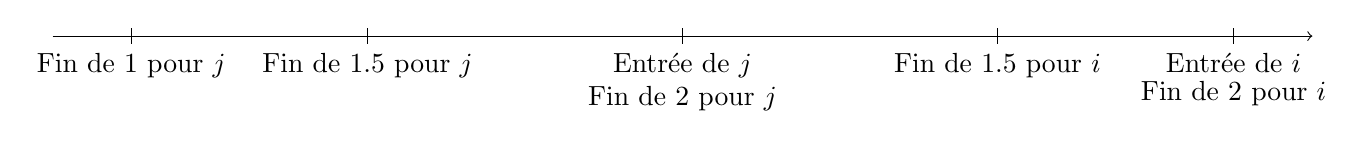
\begin{tikzpicture}
        \draw[->] (-8,0) -- (8,0) node [below] {};
        \foreach \x/\d in {-7/Fin de 1 pour $j$,-4/Fin de 1.5 pour $j$, 0/Entrée de $j$\\Fin de 2 pour $j$,4/Fin de 1.5 pour $i$,7/Entrée de $i$\\Fin de 2 pour $i$}
        \draw (\x, 0.1) -- (\x, -0.1) node [below] {\shortstack{\d}};
    \end{tikzpicture}\end{center}
    --- Fin de 1 pour $i$ avant fin de 1 pour $j$ : $i$ avait fini de choisir un ticket lorsque $j$ teste s'il est prioritaire sur $i$.\\
    --- Fin de 1 pour $i$ avant fin de 1.5 pour $j$ : absurde par le même raisonnement.\\
    --- Fin de 1 pour $i$ avant fin de 2 pour $j$ : \texttt{ticket[i] > ticket[j]}, or $j$ est prioritaire, absurde. \\
    On a donc bien exclusion mutuelle.

    Si plusieurs fils attendent, il y en a un qui est prioritare sur les autres. Il n'y a donc pas d'interblocage, ni de famine puisqu'un fil ne peut attendre qu'un nombre fini d'autres fils.
\end{prop}

\begin{prop}{}{}
    Cet algorithme a le même problème que celui de Peterson, les compilateurs peuvent le rendre faux en l'optimisant.
\end{prop}

\begin{defi}{}{}
    Ces deux méthoes font partie de l'attente active, il s'agit des procédés où l'attente est réalisée à l'aide de requêtes répétées. Cette méthode nécessite du temps de calcul. C'est une des limites de l'attente active.
\end{defi}

\begin{defi}{Attente passive.}{}
    On cherche à n'avancer les calculs dans les fils uniquement lorsque ceux-ci sont prioritaires. Ces méthodes sont souvent des appels système avec des garanties sur ceux-ci. Pour cela, on utilise des \bf{mutex}, ou \bf{verrou}. Il s'agit de booléens bloquant l'accès aux sections critiques. Ils sont dotés de deux fonctions :\\
    --- Verrouiller : tant que le verrou est verrouillé, attend puis le verrouille. Un seul fil peut verrouiller un mutex.\\
    --- Déverrouiller : libère le mutex.
\end{defi}

\begin{defi}{}{}
    En C, on utilisera le type \c{pthread_mutex_t} pour représenter un mutex.\\
    Celui-ci est muni de 4 opérations :\\
    --- \c{pthread_mutex_init(pthread_mutex_t *mutex, pthread_mutexattr_t *attr)} : initialise le mutex.\\
    --- \c{pthread_mutex_destroy(pthread_mutex_t *mutex)} : détruit le mutex.\\
    --- \c{pthread_mutex_lock(pthread_mutex_t *mutex)} : verrouille le mutex, ou se met en attente.\\
    --- \c{pthread_mutex_unlock(pthread_mutex_t *mutex)} : déverrouille le mutex s'il est dévérouillé.
\end{defi}

\begin{ex}{}{}
    Sur l'exemple du compteur, le parallélisme avec mutex est plus lent que le séquentiel. Si la proportion des fonctions en section critique était plus faible, on pourrait effectivement accélérer les calculs.
\end{ex}

\begin{defi}{Sémaphores.}{}
    Dans la vie courante, les sémaphores sont l'équivalent des feux tricolores pour les trains. C'est ce qui interdit à un train d'accéder à une portion de voie ferrée. En informatique, ce sont des verrous associés à un entier. Ce sont des structures munies de deux opérations : incrémenter et décrémenter.
\end{defi}

\begin{defi}{Problème producteur/consommateurs.}{}
    Des producteurs alimentent un stock, des consommateurs récupères des marchandises dans ce stock.\\
    Un consommateur ne peut récupérer des marchandises seulement s'il en reste dans le stock.\\
    Le sémaphore indique la quantité restante de marchandises.
\end{defi}

\begin{defi}{Utilisation en C.}{}
    En C, on utilise l'entête \c{<semaphore.h>}, on utilise des objets de type \c{sem_t}.\\
    On a accès à plusieurs fonctions :\\
    $\hra$ \c{sem_wait} : Décrémente le sémaphore, attend la permission de le faire.\\
    $\hra$ \c{sem_post} : Incrémente le sémaphore.\\
    $\hra$ \c{sem_init} et \c{sem_destroy} : initialisation et destruction du sémaphore.
\end{defi}

\begin{defi}{Barrières de synchronisation.}{}
    Il s'agit d'une portion de code qui permet aux fils de s'attendre les uns les autres.\\
    Les sémaphores ont un avantage : n'importe qui peut incrémenter le sémaphore, ce n'est pas le cas des mutex où seul celui qui a verrouillé peut le déverouiller.\\
    Pour implémenter une barrière de synchronisation, on pourrait suivre le nombre de fils qui sont en train d'attendre. On utilise une variable protégée par un mutex pour cela.\\
    Quand un fil arrive, il incrémente cette variable. Si on est le dernier, on veut en avertir les autres fils. On utilise un sémaphore incrémenté antant de fois qu'il y a de fils, et le dernier fil incrémente le sémaphore, qui était initialisé à 0. Les autres fils le décrémentent.\\
    On utilise une variable nombre\_attente initialisée à 0, un mutex verrou et un sémaphore départ.\\
    \begin{algorithm}[H]
        \caption{Barrière de synchronisation.}
        Verouiller(verrou).\\
        nombre\_attente++\\
        \Si{nombre\_attente $\neq$ p}{
            Décrementer(depart).
        }\Sinon{
            nombre\_attente $\gets$ 0.\\
            \Pour{$i$ allant de 1 à $p-1$}{
                Incrémenter(depart).
            }
        }
        Déverouiller(verrou).\\
    \end{algorithm}
    Cette barrière n'est pas réutilisables, certains fils pourraient re-rentrer avant que tous n'en soient sortis.\\
    On peut mettre en place une seconde barrière de synchronisation identique pour permettre la réutilisation.\\
    Les fils attendent en $B_1$ qu'ils aient tous finis leur tache, ils attendent en $B_2$ qu'ils aient tous franchi la barrière $B_1$.
\end{defi}

\begin{defi}{En OCaml.}{}
    En OCaml, un fil est de type $t$.\\
    $\hra$ \ocaml{Thread.create : ('a, 'b) -> 'a -> Thread.t} : crée un fil.\\
    $\hra$ \ocaml{Thread.join : Thread.t -> unit} : attend la fin du fil.\\
    $\hra$ \ocaml{Mutex.create : unit -> Mutex.t} crée un mutex.\\
    $\hra$ \ocaml{Mutex.lock : Mutex.t -> unit} : verrouille le mutex.\\
    $\hra$ \ocaml{Mutex.unlock : Mutex.t -> unit} : déverrouille le mutex.
\end{defi}

\end{document}